\documentclass[12pt]{article}

\usepackage{CJKutf8}
% 打中文時請務必加這個Package

\usepackage{epsfig,amsmath,amssymb,latexsym}
\usepackage{graphicx,epsfig,color,epsf,psfrag,hhline,amsmath,amssymb,textcomp}
\usepackage{hyperref}
\usepackage{enumitem}

\setlength {\topmargin}{-1.0in}
\setlength {\textheight}{10in}
\setlength {\oddsidemargin}{-0.25in}
\setlength {\evensidemargin}{-0.25in}
\setlength {\textwidth}{6.75in}
\setlength {\parskip}{8pt plus 2pt minus 1pt}

\newtheorem{theorem}{Theorem}[section]
\newtheorem{definition}{Definition}[section]
\newtheorem{lemma}{Lemma}[section]

\newcommand{\comb}[2]{\left (\begin{array}{c} #1 \\ #2 \end{array} \right )}

\newcommand{\inlinecomb}[2]{\mbox{\scriptsize $\left (\begin{array}{c} #1 \\ #2 \end{array} \right )$\normalsize}}

\newcommand {\bsolution}{\noindent {\em Solution:} \ }

\newcommand{\esolution}{\hfill $\Diamond$ \\ \vspace{.3cm}}

%************************** Figure**********************************
\newcommand {\bfig}[2] {\begin{figure}[htbp]
                        \centerline {
                         \epsfig{figure={#1},clip=,width={#2}}}}

\newcommand {\efig}[2]{ \caption{#2}
                        \label{fig:#1}
                        \end{figure}
                        \mymarginpar{fig:#1}}
\newcommand {\rfig}[1]{Figure \ref{fig:#1}}

%%%%%%%%%%%%%%%%%%%%%%%%%%%%%%%%%%%%%%%%%%%%%%%%%

\begin{document}
\thispagestyle{empty}
\begin{center}
{\Large \noindent COM 530500 {\bf Network Science Homework \#1} \\
\large {{\sc Due:} Thursday, October 14, 2021}  \\
}
\emph{No late homework will be accepted}.
\end{center}


\noindent {\begin{CJK}{UTF8}{bsmi}
{\bf 班級:} 資應所
\end{CJK}}

\noindent  {\begin{CJK}{UTF8}{bsmi}
{\bf 姓名:} 鄭程哲
\end{CJK}}

\noindent {\begin{CJK}{UTF8}{bsmi}
{\bf 學號:} 110065512
\end{CJK}}

\bigskip

%---------------------------------------------------------------------------
% Problem 1
%---------------------------------------------------------------------------
\begin{figure}[h]
	\centering
	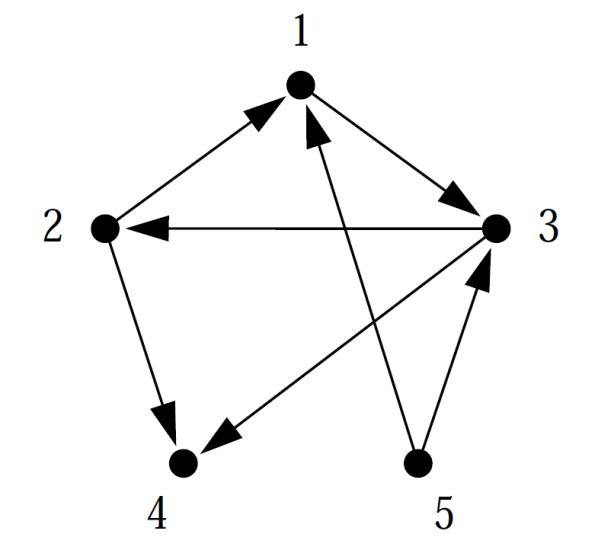
\includegraphics[width=0.4\textwidth]{NS_Hw1_a.jpg}
	\caption{Network (a).}
	\label{NS_Hw1_a}
\end{figure}

\noindent {\bf Problem 1.\bf(10\%)}
\begin{enumerate}[label=(\alph*)]
	\item (5\%) Write down the adjacency matrix of network (a).
	\item (5\%) Write down the cocitation matrix of network (a).
\end{enumerate}

\bsolution
%---------------------------------------------------------------------------

(a) $\begin{bmatrix}
	0 & 1 & 0 & 0 & 1 \\
	0 & 0 & 1 & 0 & 0 \\
	1 & 0 & 0 & 0 & 1 \\
	0 & 1 & 1 & 0 & 0 \\
	0 & 0 & 0 & 0 & 0 
	\end{bmatrix}$

(b) Cocitation matrix $C = AA^{T} = \begin{bmatrix}
	2 & 0 & 1 & 1 & 0 \\
	0 & 1 & 0 & 1 & 0 \\
	1 & 0 & 2 & 0 & 0 \\
	1 & 1 & 0 & 2 & 0 \\
	0 & 0 & 0 & 0 & 0
\end{bmatrix}$
%---------------------------------------------------------------------------
\esolution

%---------------------------------------------------------------------------
% Problem 2
%---------------------------------------------------------------------------
\begin{figure}[h]
	\centering
	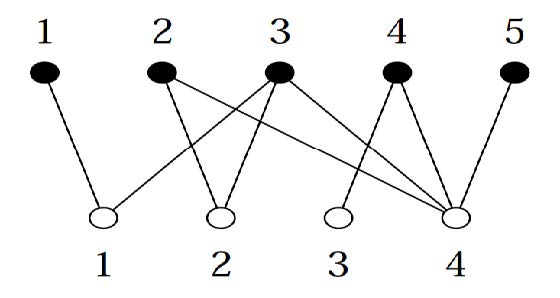
\includegraphics[width=0.4\textwidth]{NS_Hw1_b.jpg}
	\caption{Network (b).}
	\label{NS_Hw1_b}
\end{figure}

\noindent {\bf Problem 2.\bf(10\%)}
\begin{enumerate}[label=(\alph*)]
	\item (5\%) Write down the incidence matrix of network (b).
	\item (5\%) Write down the projection matrix for the projection of network (b) onto its black vertices.
\end{enumerate}

\bsolution
%---------------------------------------------------------------------------

(a) I regard white dots as different groups and black dots as vertexs.\\
	Incidence matrix = $B = \begin{bmatrix}
	1 & 0 & 1 & 0 & 0 \\
	0 & 1 & 1 & 0 & 0 \\
	0 & 0 & 0 & 1 & 0 \\
	0 & 1 & 1 & 1 & 1 
\end{bmatrix}$


(b) Projection matrix $P = B^{T}B =\begin{bmatrix}
	1 & 0 & 1 & 0 & 0 \\
	0 & 2 & 2 & 1 & 1 \\
	1 & 2 & 3 & 1 & 1 \\
	0 & 1 & 1 & 2 & 1 \\
	0 & 1 & 1 & 1 & 1
	\end{bmatrix} $

%---------------------------------------------------------------------------
\esolution


%---------------------------------------------------------------------------
% Problem 3
%---------------------------------------------------------------------------

\noindent {\bf Problem 3.\bf(10\%)}
Consider a bipartite network, with its two types of vertices. Suppose there are $n_1$ vertices of type $1$ and $n_2$ vertices of type $2$. Show that the mean degrees $c_1$ and $c_2$ of the two types are related by $c_2=\frac{n_1}{n_2}c_1$.

\bsolution
%---------------------------------------------------------------------------
If there are $m$ edges between two types of vertices, The mean degree of type 1 vertices\\[0.6em]
$c_1=\frac{m}{n_1}$, and $c_2=\frac{m}{n_2}$. Therefore, 
$\frac{c_1}{c_2}=\frac{\frac{m}{n_1}}{\frac
	{m}{n_2}}=\frac{n_2}{n_1}$, and we get 
$c_2=\frac{n_1}{n_2}c_1$.
%---------------------------------------------------------------------------
\esolution

%---------------------------------------------------------------------------
% Problem 4
%---------------------------------------------------------------------------
\noindent {\bf Problem 4.\bf(20\%)}
Given 
	\[A=
		\begin{pmatrix}
			0 & 2 & -1 \\
			2 & 3 & -2 \\
			-1 & -2 & 0
		\end{pmatrix},
	\]

\begin{enumerate}[label=(\alph*)]
	\item (10\%) Find all eigenvalues of matrix $A$.
	\item (10\%) Find an orthogonal matrix $U$ that diagonalizes $A$.
\end{enumerate}

\bsolution
%---------------------------------------------------------------------------

(a) Eigenvalues can be obtained by the equation: $Ax=\lambda x$, 
and $(A-\lambda I)$ is a singular matrix. Therefore, $det(A-\lambda I)=0$. \\
\[det(A-\lambda I)=det
	\begin{pmatrix}
		0-\lambda & 2 & -1 \\
		2 & 3-\lambda & -2 \\
		-1 & -2 & 0-\lambda
	\end{pmatrix}=0
\]
\[-\lambda^3+3\lambda^2+9\lambda+5=0\]
\[Eigenvalues(\lambda)= -1, -1, 5\]

(b) Orthogonal matrix is composed by eigenvectors of $A$.
\begin{enumerate}
	\item When $\lambda=-1, A-(-1)I=
	\begin{pmatrix}
		1 & 2 & -1 \\
		2 & 4 & -2 \\
		-1 & -2 & 1
	\end{pmatrix}\sim
	\begin{pmatrix}
		1 & 2 & -1 \\
		0 & 0 & 0 \\
		0 & 0 & 0
	\end{pmatrix}$. So a normalized eigenvector for $\lambda _1=-1$ is 
	$v_1=(\frac{1}{\sqrt{2}}, 0, \frac{1}{\sqrt{2}})$.
	\item When $\lambda=5, A-(5)I=
	\begin{pmatrix}
		-5 & 2 & -1 \\
		2 & -2 & -2 \\
		-1 & -2 & -5
	\end{pmatrix}\sim
	\begin{pmatrix}
		1 & -1 & -1 \\
		-5 & 2 & -1 \\
		-1 & -2 & -5
	\end{pmatrix}\sim
	\begin{pmatrix}
		1 & 0 & 1 \\
		0 & 1 & 2 \\
		0 & 0 & 0
	\end{pmatrix}$. So a normalized eigenvector for $\lambda _1=-1$ is 
	$v_1=(\frac{-1}{\sqrt{6}}, \frac{-2}{\sqrt{6}}, \frac{1}{\sqrt{6}})$.
\end{enumerate}
\qquad\quad Finally, orthogonal matrix $U=
	\begin{pmatrix}
		\frac{1}{\sqrt{2}} & \frac{1}{\sqrt{2}} & \frac{-1}{\sqrt{6}} \\[0.4em]
		0 & 0 & \frac{-2}{\sqrt{6}} \\[0.4em]
		\frac{1}{\sqrt{2}} & \frac{1}{\sqrt{2}} & \frac{1}{\sqrt{6}}
	\end{pmatrix}$.
%---------------------------------------------------------------------------
\esolution

%---------------------------------------------------------------------------
% Problem 5
%---------------------------------------------------------------------------
\noindent {\bf Problem 5.\bf(15\%)}
Read the tutorial from \href{https://github.com/PingEnLu/Network-Science-COM530500/tree/master/Network_Science_Python_iGraph_Tutorial}{Ping-En Lu's GitHub repository} to install Python3 and python-igraph (if you need).

Paste your screenshots of “Hello, World!” of both Python 3 (5\%) and python-igraph (5\%), and write a brief report (5\%). (For example, you can write down some problems you encountered, and how you solved them.)

\bsolution
%---------------------------------------------------------------------------
I didn't encounter any problem during the installation of both Python and Python-iGraph.
Additionally, I didn't meet the issue the tutorial has mentioned about installing Python-iGraph on Windows. I installed it directly by typing pip command in command line.

\begin{figure}[h]
	\centering
	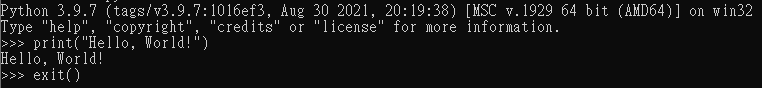
\includegraphics[width=0.9\textwidth]{fig-prob5-python.png}
	\caption{Python screenshot.}
	\label{HW1_5_python}
\end{figure}
\begin{figure}[h]
	\centering
	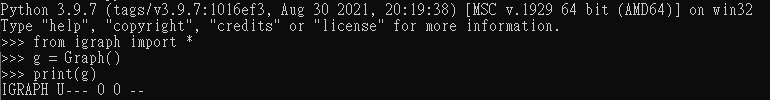
\includegraphics[width=0.9\textwidth]{fig-prob5-igraph.png}
	\caption{Python-iGraph screenshot.}
	\label{HW1_5_igraph}
\end{figure}
%---------------------------------------------------------------------------
\esolution
\newpage

%---------------------------------------------------------------------------
% Problem 6
%---------------------------------------------------------------------------
\noindent {\bf Problem 6.\bf(35\%)}
Please download the {\bf tvshow} dataset from \href{https://github.com/PingEnLu/Network-Science-COM530500/tree/master/Network_Science_Python_iGraph_Tutorial}{Ping-En Lu's GitHub repository}, and find the following information from this dataset.

\begin{itemize}
	\item Number of nodes. (5\%)
	\item Number of edges. (5\%)
	\item Mean degree. (5\%)
	\item Maximum degree. (5\%)
	\item Diameter. (5\%)
\end{itemize}
You need to upload your {\bf python source code} to iLMS, and {\bf write a brief report (10\%) including screenshots, README file, and descriptions of your code} below the solution area. There will be no points for this problem if you do not upload your python source code to iLMS.

\bsolution
%---------------------------------------------------------------------------
\begin{itemize}
	\item Number of nodes: 3892
	\item Number of edges: 8631
	\item Mean degree: 4.4352517985611515
	\item Maximum degree: 67
	\item Diameter: 28
\end{itemize}
My code is divided into two major part. The first part is to create whole graph by the dataset. I used a loop to read each row and add vertices and edges in the graph. The second part is to output the reslut. Because iGraph is powerful and very convenience, I simply called built-in methods to get the information I need. 
\begin{figure}[h]
	\centering
	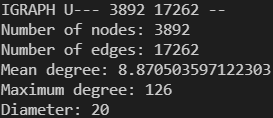
\includegraphics[width=0.5\textwidth]{fig-prob6.png}
	\caption{Result screenshot.}
	\label{HW1_6}
\end{figure}
%---------------------------------------------------------------------------
\esolution

%---------------------------------------------------------------------------
% The end of problems.
%---------------------------------------------------------------------------


\end{document}
